% Engelschulung 34c3

% kann sein wir haben gar keine Slides beim Vortrag weil die Saal-Technik zickt

% unterschiedliche Coding-Stile vorhanden wegen unterschiedlicher Autoren

\documentclass[hyperref={pdfpagelabels=false},aspectratio=169]{beamer}
\setbeamertemplate{navigation symbols}{}    % macht hässlich weg
\setbeamertemplate{itemize item}{$\bullet$}  % macht anderes hässlich weg
\usepackage{lmodern}
\usepackage[utf8]{inputenc}
\hypersetup{urlcolor=blue}
\urlstyle{sf}

\title{Engelschulung}    % Benjamin findet das Wort gehört zur Folklore und ist erfrischend  nicht-polished
\author{c3voc}   % wer will noch persönlich genannt werden?
\date{\today} 

\begin{document} % vor dem Vortrag/Test ob Beamer geht
\begin{frame}
\titlepage
\end{frame} 


\begin{frame}  
\tableofcontents
\end{frame} 
% "Welcome to the audio/video-introduction! <Leute Vorstellen> 
% Who of you is new to this? Even if have attended audio-video-introductions before, stay tuned, some tings will be different than last year."

\section{Gear}  % Sophie
\subsection{Cameras}
\begin{frame}{Cameras}
	\begin{columns}[T,onlytextwidth]
	\column{0.4\textwidth}
	\begin{figure} 
		\centering
		\def\svgwidth{1\textwidth}
		\input{camera-controls.pdf_tex}
	\end{figure}
	\column{0.6\textwidth}
	Cameras are in manual mode because of difficult lighting situation.
	\begin{description}
		\item[Left Ring] Focus - control sharpness of the image.
		\item[Middle Ring] Zoom - vary the focal length.
		\item[Right Ring] Iris - don't touch.
     \end{description}
\end{columns}
\end{frame}

\begin{frame}{Tripod Handle Controls}
	\begin{columns}[T,onlytextwidth]
	\column{0.4\textwidth}
	\begin{figure} 
		\centering
		\includegraphics[width=0.8\textwidth]{tripod-handle.jpeg}
	\end{figure}
	\column{0.6\textwidth}
	Beware: various models in use.
	\begin{description}
		\item[Zoom Control] lever above red ring
		\item[Red Button] Start/stop recording, don't touch
		\item[Other Buttons] markings on the handle
    \end{description}
	\end{columns}
\end{frame}

\begin{frame}{Tripod}
	\begin{columns}[T,onlytextwidth]
	\column{0.4\textwidth}
	\begin{figure} 
		\centering
		\includegraphics[width=1\textwidth]{tripod-complete.png}
	\end{figure}
	\column{0.6\textwidth}
	\begin{itemize}
	\item Variable brakes
 	\item Tilt axis: balanced via spring
 	\item Pan axis: smooth pans over the entire stage.
		\end{itemize}
	\end{columns}
\end{frame}

\subsection{Voctomix} % Sophie
\begin{frame}{Voctomix}
	\begin{figure} 
		\centering
		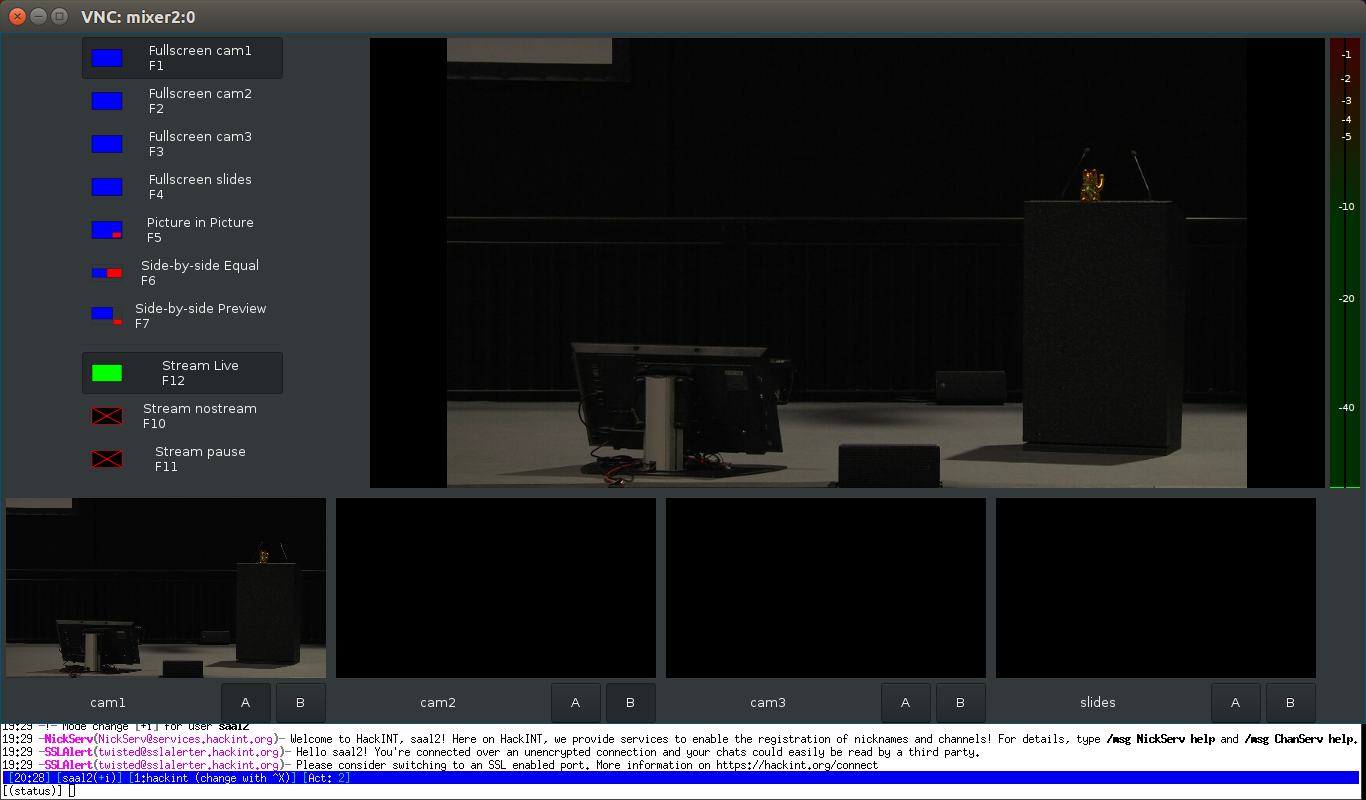
\includegraphics[width=0.8\textwidth]{voctomix.png}
	\end{figure}
\end{frame}

\begin{frame}{Composition modes}
	\begin{figure} 
		\centering
		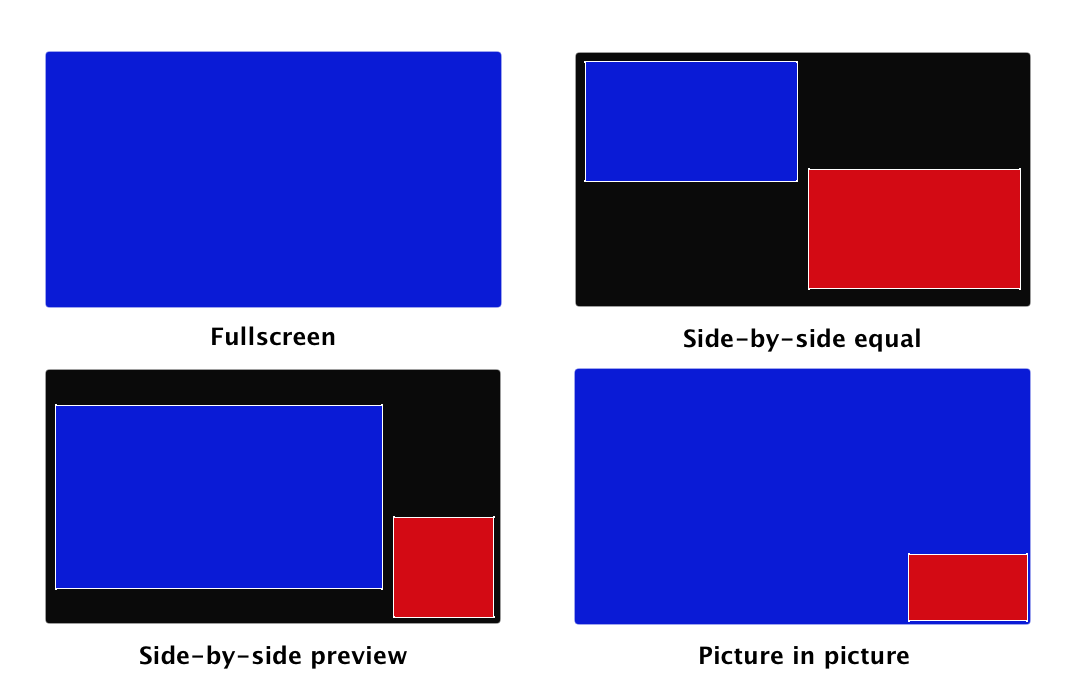
\includegraphics[width=0.8\textwidth]{composition_modes.png}
	\end{figure}
\end{frame}


\subsection{Intercom} %?
 	\begin{frame}{Intercom}
 	\begin{itemize}
 		\item Cameras: Headset + Bodypack
 		\item Mixer Desk: Communication Panel
 	\end{itemize}
 	\end{frame}

\subsection{Stream-Observer-Software} %Frederick
\begin{frame}{Stream-Observer-Software}
\begin{itemize}
\item die Stream Observer App  ist ganz toll und wird von Frederik vorgestellt
\item  (placeholder)
\end{itemize}
\end{frame}

\section{Timeline of a talk}  % Benjamin
\subsection{Before}
\begin{frame}{Before the talk}
\begin{itemize} %[<+->] später wieder einfliegend machen
\item be on time % the venue is large, please make sure that you arrive on time
\item check in with angels % meet at the mixeer desk, is everybody there? if yes camera angels go to cameras and everybody starts using intercom, if not camm heaven für replacement  
\item check hardware % do the cameras and mixer desl work as expected? if something is wrong get help from AV-tecnician  
\item evaluate skill level and vocabulary % the mixer angel has to figure out how good the camera angels can film, talk to each other and make sure everybody understands the same words.  
\item [($\bullet$] mixer angel checks slides) % if you still have time and if the speaker looks like they have capacity for it, the mixer angel takes a look at the slides to figure out whether or not to use picture-in-picture or superscource in this talk.
% I would recommend to NOT ask the speaker where they walk around on stage. Usually they don't give a useful answer and if they do they are highly professional and easy to film anyway. The speakers have to focus on the content and their way of speaking, where they walk around on stage is a minor issue. If you want to estimate how a speaker will behave on stage, check them out on youtube.
\item set stream live % set stream live, heralds want to be on the stream
\end{itemize} 
\end{frame}

\subsection{During} % Benjamin
\begin{frame}{During the talk}
\begin{itemize}
\item talk to each other % talk to each other on the intercom! there are little hard rules for that like the camera angel has to know when they are 
\item show slides immediately
\item read slides twice
\item don't film the audiance
\item this is a lecture, not an action-movie 
\item if problem, talk to A/V-technician
\item different image for camera 1 and 2, camera 1 does close-up
\end{itemize} 
\end{frame}


\begin{frame}{Image composition}
	\begin{columns}[T,onlytextwidth]
	\column{0.5\textwidth}
	\begin{figure} 
		\centering
		\def\svgwidth{1\textwidth}
		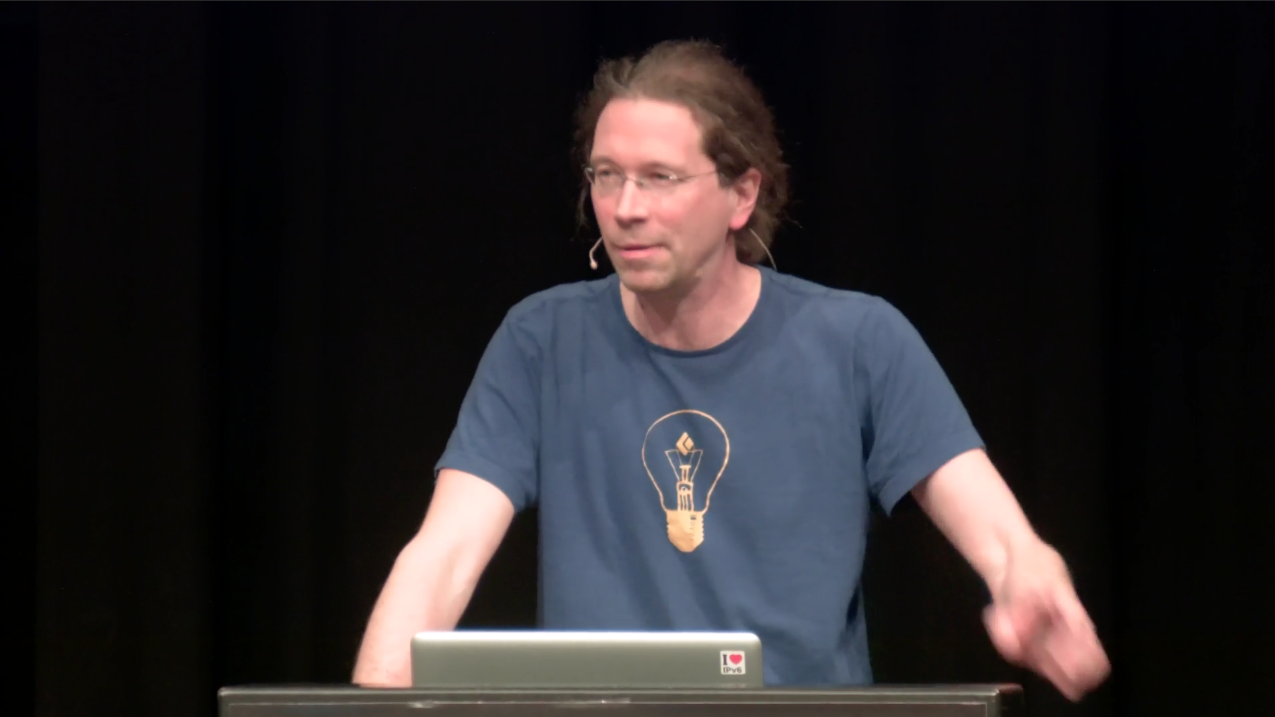
\includegraphics[width=0.9\textwidth]{closeup.png} \\camera 1
	\end{figure}
\column{0.5\textwidth}
	\begin{figure} 
		\centering
		\def\svgwidth{1\textwidth}
		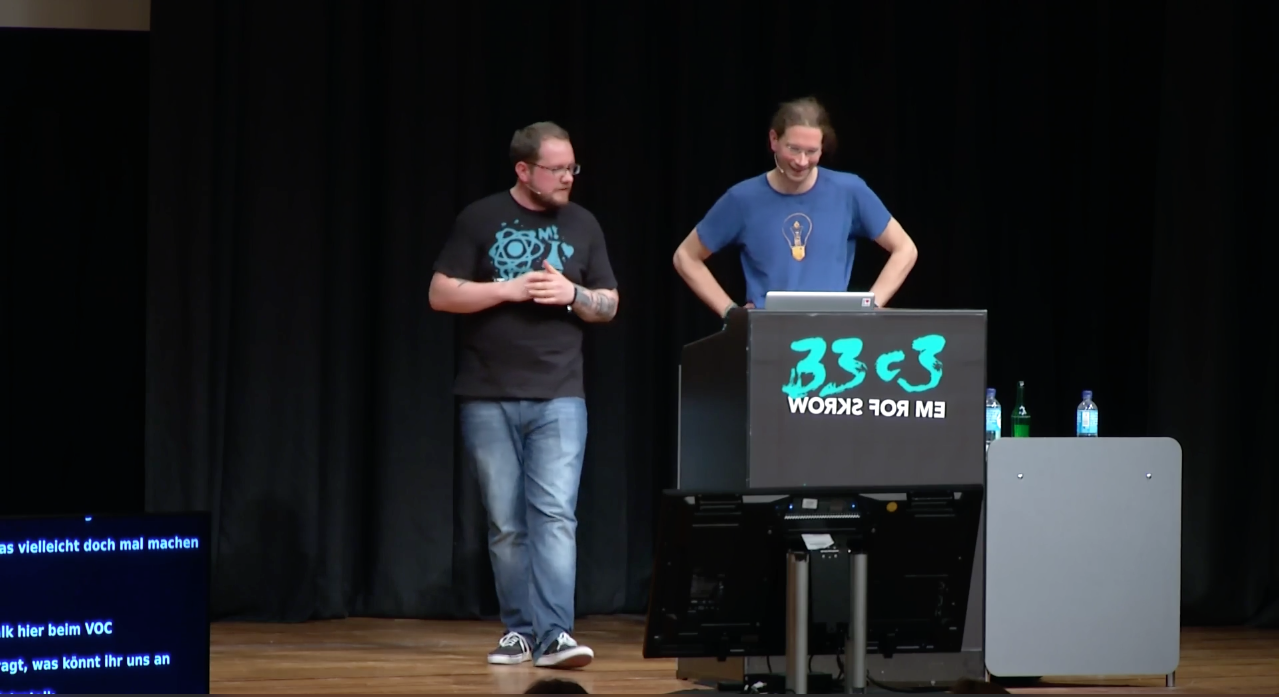
\includegraphics[width=0.93\textwidth]{medium.png} \\camera 2
	\end{figure}
\end{columns}
\end{frame}


\begin{frame}
	\begin{columns}[T,onlytextwidth]
	\column{0.5\textwidth}
	\begin{figure} 
		\centering
		\def\svgwidth{1\textwidth}
		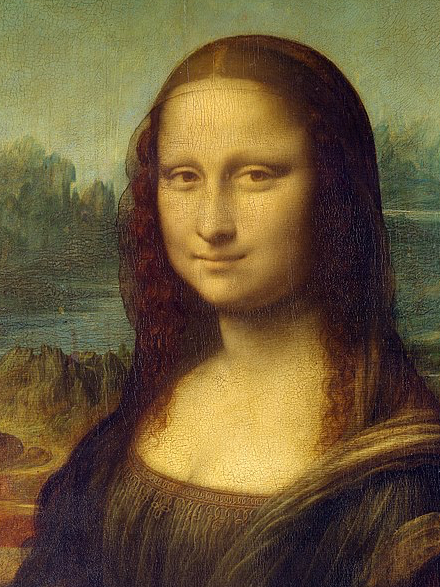
\includegraphics[width=0.7\textwidth]{in_bild_gucken.jpg} \\
		\textcolor{green}{\textbf{yes}}	
	\end{figure}
\column{0.5\textwidth}
	\begin{figure} 
		\centering
		\def\svgwidth{1\textwidth}
		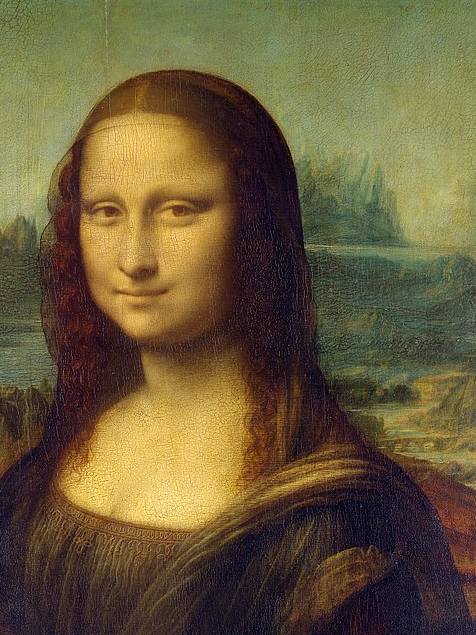
\includegraphics[width=0.7\textwidth]{aus_bild_gucken.jpg} \\
		\textcolor{red}{\textbf{no}}	
	\end{figure}
\end{columns}
\end{frame}


\begin{frame}
	\begin{columns}[T,onlytextwidth]
	\column{0.3\textwidth}
	\begin{figure} 
		\centering
		\def\svgwidth{1\textwidth}
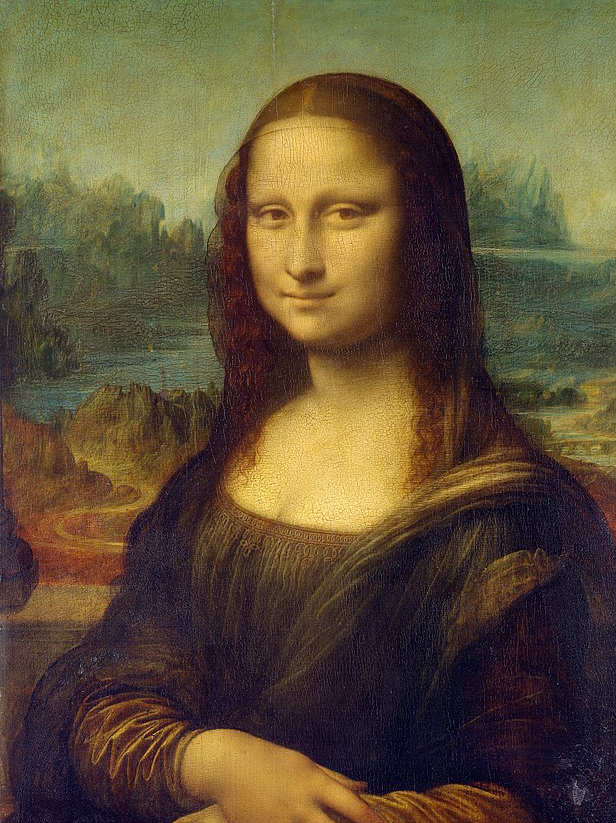
\includegraphics[width=1\textwidth]{haende_ab.jpg} \\
		\textcolor{red}{\textbf{no}}	\\(half hands or feet)
	\end{figure}
	\column{0.3\textwidth}
	\begin{figure} 
		\centering
		\def\svgwidth{1\textwidth}
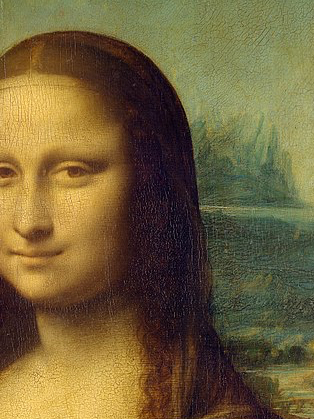
\includegraphics[width=1\textwidth]{kopf_halb.jpg} \\
		\textcolor{red}{\textbf{no}}	\\(half head)
	\end{figure}
\column{0.3\textwidth}
	\begin{figure} 
		\centering
		\def\svgwidth{1\textwidth}
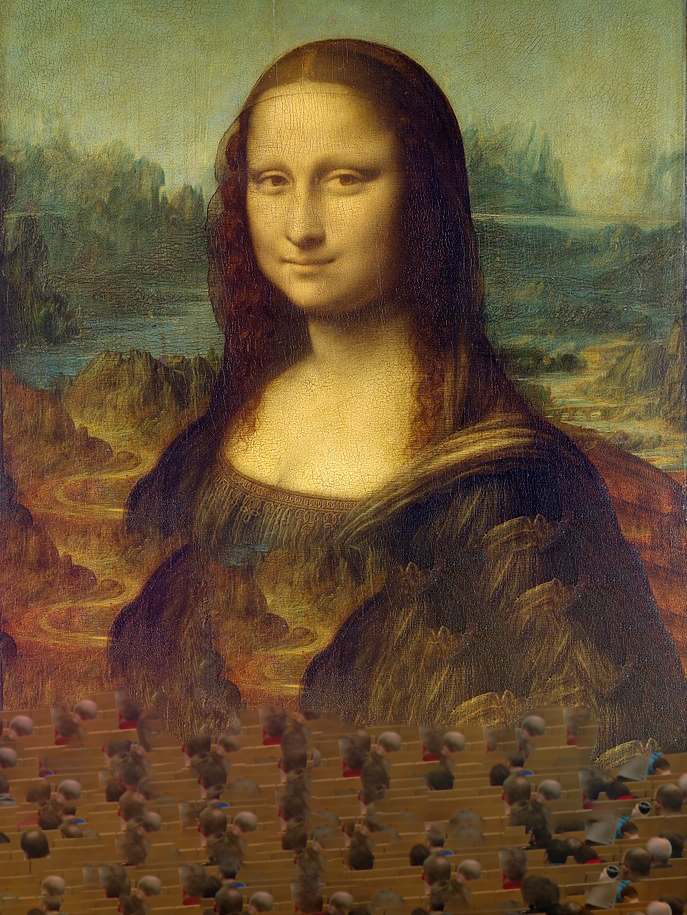
\includegraphics[width=1\textwidth]{audience.jpg} \\
		\textcolor{red}{\textbf{no}}	\\(audience)
	\end{figure}
\end{columns}
\end{frame}

\begin{frame}
	\begin{columns}[T,onlytextwidth]
	\column{0.5\textwidth}
	\begin{figure} 
		\centering
		\def\svgwidth{1\textwidth}
		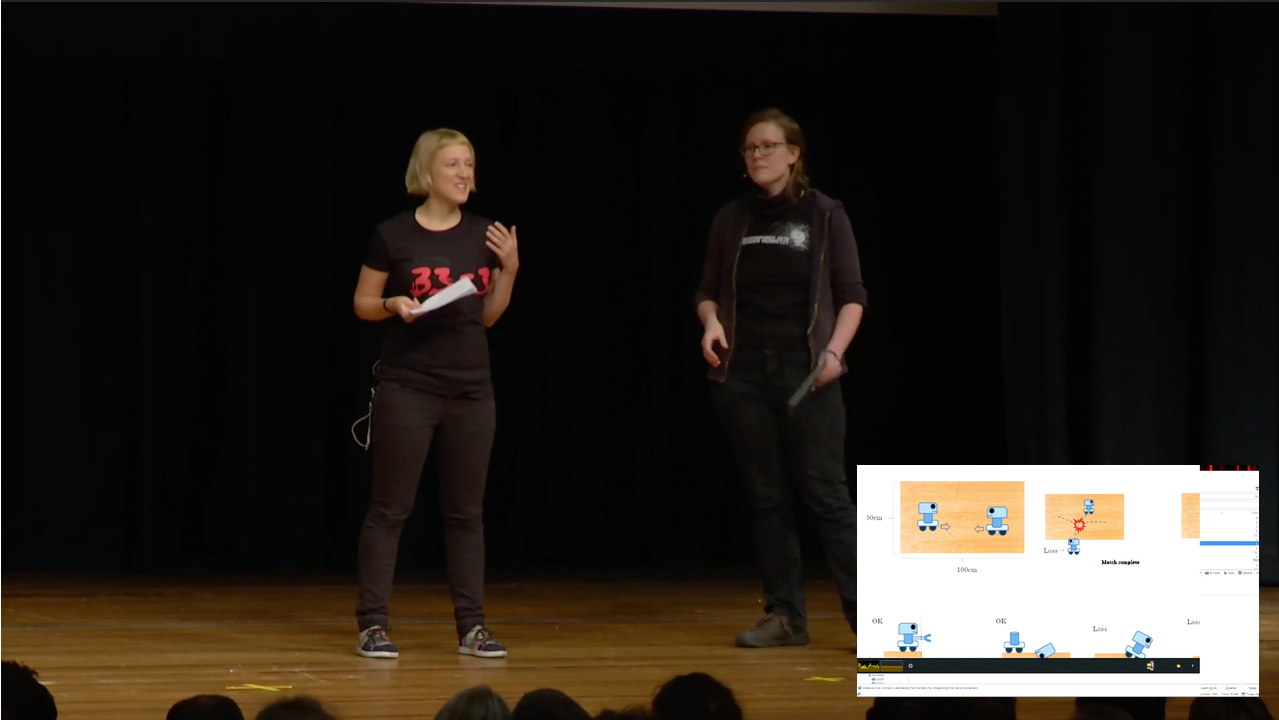
\includegraphics[width=1\textwidth]{ssrcfckup.png} \\
		\textcolor{red}{\textbf{no}}	
	\end{figure}
	\column{0.5\textwidth}
	\begin{figure} 
		\centering
		\def\svgwidth{1\textwidth}
		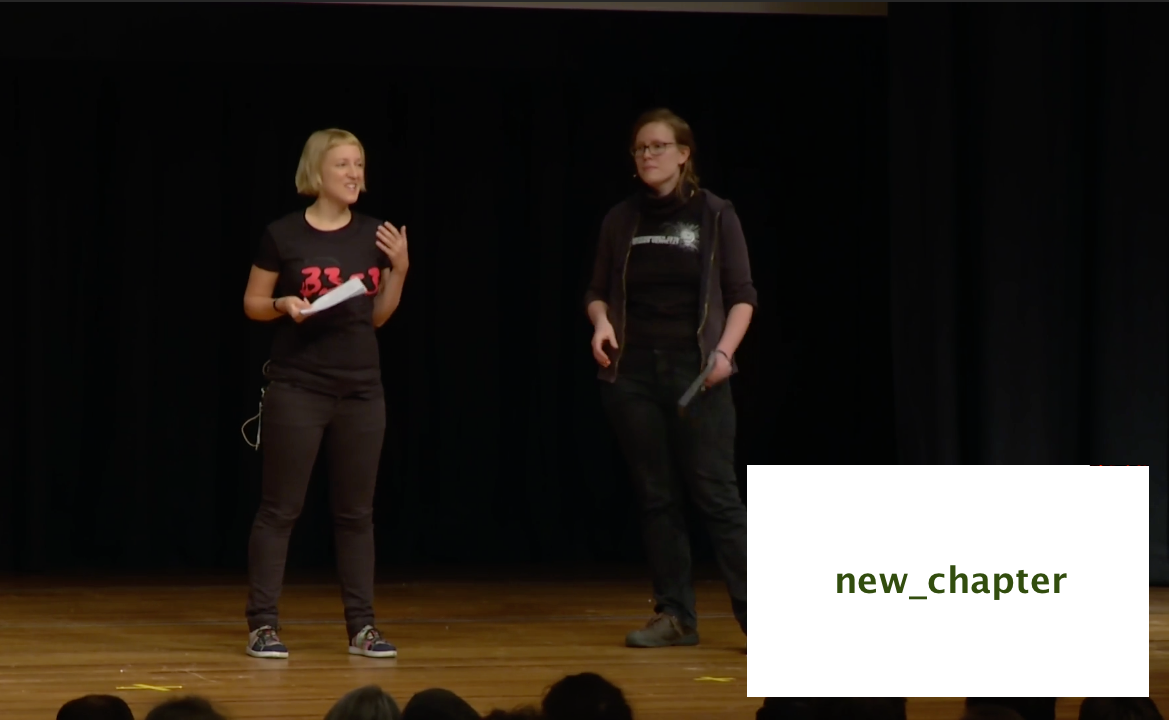
\includegraphics[width=0.92\textwidth]{ssrcbetter.png} \\
		\textcolor{green}{\textbf{yes}}	
	\end{figure}
\end{columns}
\end{frame}


\subsection{After} % Benjamin
\begin{frame}
\frametitle{After the talk}
\begin{itemize}
\item thank each other, for further feedback you might meet at the mixer desk
\end{itemize} 
\end{frame}


\subsection{Meanwhile ... stream observing angels} % Frederik + Capo
\begin{frame}{Stream observing angels}
\begin{itemize}
\item  ganz super sache
\item  (placeholder)
\end{itemize} 
\end{frame}

\section{Quality}  %Benjamin
\subsection{Making shit great again} 
\begin{frame}
\end{frame}
% <Benjamin> And then there is the thing with the quality. In the past years the quality of the recordings we produce got better and so developed the expectations. We still have the problems that not all angels deliver the quality that the VOC would like to see. Now, we already spoke about what things we’d like to see, but … <points to empty slides> oops, what is that? A blank slide? <break> I actually once had a talk where the speaker had blank slides when she would speak and there was nothing visual to show. Which from a performance-perspective I find quite obvious. You listen to my voice now, if it was in a dark theatre, seeing and hearing me would be the only source of information, I would have more of your arrention than with a projected image. But as a mixer angel I was fucked, because I was conditioned to always go on the slides when a new slide appears and my conditioning was in the way. Suddenly I was the problem. <break> What I’m trying to say here is that how talks become complicated comes unexpectedly, sometimes the speaker is the problem, sometimes the equipment is the problem, and sometimes you are the problem. All of us. We cannot cover all complicated cases in the Engelschulung but we have to encourage you to be the best camera- stream-observer- and mixer angel that you can be. So here are a few things that you can do.


\begin{frame}{Quality}
\begin{itemize} %[<+->]
\item hands-on training with Frederik and Allan % go to the hads-on training with Frederik 
\item do stream-observer shifts % do stream-observer shifts, especially if you ar a beginner
\item get feedback from peers % feedback with peers, do it with a friend, one is doing the editing and the other the stream observing and afterwards you talk how it went
\item get feedback from Capo % <macht Capo selber>
\item watch your own edits (post event) % watch your own edits after the event, at least a bit, so you have an idea how you performed
\item do it more than once a year, check 
\textcolor{blue}{\textbf{c3voc.de/wiki }} % do it more than once a year! You can check out in the VOC-Wiki where other events are where the VOC is doing video, if you do it more often you won't forget it until next congress
\item have a habit of continuous improvement % this is for everybody, having a habit of continuous improvement. if you think you know how video editing works, you are probably part of the problem. please, everybody should strive to get better, there is always something to improve. During the shift-distribution meeting I'd actually like to ask some people "what was the last thing you've learnt that you'll make better next time", and you better have an answer.
\end{itemize} 
\end{frame}

\section{Orga} % Alex
\subsection{Meetings}
\begin{frame}{Daily Meeting}
\begin{itemize}
\item  We meet, in \textbf{Lecture Room 11}, times can be found at 
\renewcommand\UrlFont{\color{blue}\sffamily\textbf} 
\url{events.ccc.de/congress/2017/wiki/index.php/Session:A/V_Angel_Meeting}
\item  \textbf{Mandatory} for \textbf{Video Mixing Angels}
\item  \textbf{Optional} for \textbf{other A/V Angels}
\item  Feedback and Shift Distribution
\end{itemize} 
\end{frame}


\begin{frame}{Feedback Meeting}
\begin{itemize}
	\item Announcements
	\item Remarkable Examples
	\item Short Feedback Round 
\end{itemize} 
\end{frame}
% mündlich: \item First Slot of the meeting     

\begin{frame}{Shift Distribution}
\begin{itemize}
	\item Pre-Signup via Pad (do not remove others) % -> link?
	\item Commitment in Meeting % ja, da wird diskutiert aber das muss nicht auf die folien
	\item Talks with special requirements will be done in cooperation team members % ist das ein vollständiger Satz?
\end{itemize} 
\end{frame}
% mündlich: 	\item Everyone should do at least one shift per day


\subsection{Contacts}
\begin{frame}{Who to Contact?}
\begin{itemize}
\item Technical problem \textbf{in the hall} - A/V Technician on duty
\item Organization or social problems - VOC Angel Coordination - DECT \textbf{1607}
\item Further training - Frederik and Capo
\item General Angel Topics - Heaven
\item Unable to find right person for issue - VOC Angel Coordination
\item We might need to call you. Please have your DECT or UMTS number in the Engelsystem! If you don't have a number yet, go to 
\textcolor{blue}{\textbf{eventphone.de}} and get one. 
\end{itemize} 
\end{frame}
% mündlich: in person, via dect or via engelsystem
% if there is anything, please let us know.


% And now we have Q&A, do you have questions?

\end{document}